% Sandia National Laboratories is a multimission laboratory managed and
% operated by National Technology & Engineering Solutions of Sandia, LLC, a
% wholly owned subsidiary of Honeywell International Inc., for the U.S.
% Department of Energy’s National Nuclear Security Administration under
% contract DE-NA0003525.

% Copyright 2002-2019 National Technology & Engineering Solutions of Sandia,
% LLC (NTESS).


\begin{Device}\label{D_DEVICE}

\symbol
{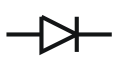
\includegraphics{diodeSymbol}}

\device
D<name> <(+) node> <(-) node> <model name> [area value]

\model
.MODEL <model name> D [model parameters]

\examples
\begin{alltt}
  DCLAMP 1 0 DMOD
  D2 15 17 SWITCH 1.5
\end{alltt}

\parameters
\begin{Parameters}

\param{\vbox{\hbox{(+) node\hfil}\hbox{(-) node}}}

The anode and the cathode.

\param{area value} 

Scales IS, ISR, IKF, RS, CJO, and IBV, and has a default value of 1.
IBV and BV are both specified as positive values.

\end{Parameters}

\comments

The diode is modeled as an ohmic resistance (\texttt{RS/area}) in series
with an intrinsic diode.  Positive current is current flowing from the
anode through the diode to the cathode. 

The power through the diode is calculated 
with $I \cdot \Delta V$ where the voltage drop is calculated as $(V_+ - V_-)$ 
and positive current flows from $V_+$ to $V_-$.  This formula may differ from
other simulators, such as HSPICE.

\end{Device}

\paragraph{Diode Operating Temperature}
\index{diode!operating temperature} Model parameters can be assigned unique
measurement temperatures using the \textrmb{TNOM} model parameter.

\paragraph{Diode level selection}

Three distinct implementations of the diode are available.  These are
selected by using the \verb|LEVEL| model parameter.  The default
implementation is based on SPICE 3F5, and may be explicitly specified
using \verb|LEVEL=1| in the model parameters, but is also selected if no
\verb|LEVEL| parameter is specified.  The PSpice implementation
~\cite{PSpiceUG:1998} is obtained by specifying \verb|LEVEL=2|.
The \Xyce{} \verb|LEVEL=200| diode is the JUNCAP200 model.

The \Xyce{} \verb|LEVEL=1| and \verb|LEVEL=2| diodes have a parameter,
\textrmb{IRF}, that allows the user to adjust the reverse current from the basic
SPICE implementation.  The usual SPICE treatment defines the linear
portion of the reverse current in terms of IS which is defined by the
forward current characteristics.  Data shows that often the reverse
current is quite far off when determined in this manner.  The
parameter \textrmb{IRF} is a multiplier that can be applied to adjust the linear
portion of the reverse current.


\pagebreak

\paragraph{Level 1 and 2 Diode Instance Parameters}
% This table was generated by Xyce:
%   Xyce -doc D 1
%
\index{diode!device instance parameters}
\begin{DeviceParamTableGenerated}{Diode Device Instance Parameters}{D_1_Device_Instance_Params}
AREA & Area scaling value (scales IS, ISR, IKF, RS, CJ0, and IBV) & -- & 1 \\ \hline
IC &  & -- & 0 \\ \hline
LAMBERTW & Option to solve diode equations with the Lambert-W function & logical (T/F) & 0 \\ \hline
OFF & Initial voltage drop across device set to zero & logical (T/F) & 0 \\ \hline
TEMP & Device temperature & -- & Ambient Temperature \\ \hline
\end{DeviceParamTableGenerated}


\paragraph{Level 1 and 2 Diode Model Parameters}
% This table was generated by Xyce:
%   Xyce -doc D 1
%
\index{diode!device model parameters}
\begin{DeviceParamTableGenerated}{Diode Device Model Parameters}{D_1_Device_Model_Params}
AF & Flicker noise exponent & -- & 1 \\ \hline
BV & Reverse breakdown "knee" voltage & V & 1e+99 \\ \hline
CJ & Zero-bias p-n depletion capacitance & F & 0 \\ \hline
CJ0 & Zero-bias p-n depletion capacitance & F & 0 \\ \hline
CJO & Zero-bias p-n depletion capacitance & F & 0 \\ \hline
EG & Bandgap voltage (barrier height) & eV & 1.11 \\ \hline
FC & Forward-bias depletion capacitance coefficient & -- & 0.5 \\ \hline
IBV & Reverse breakdown "knee" current & A & 0.001 \\ \hline
IBVL & Low-level reverse breakdown "knee" current (level 2) & A & 0 \\ \hline
IKF & High-injection "knee" current (level 2) & A & 0 \\ \hline
IRF & Reverse current fitting factor & -- & 1 \\ \hline
IS & Saturation current & A & 1e-14 \\ \hline
ISR & Recombination current parameter (level 2) & A & 0 \\ \hline
JS & Saturation current & A & 1e-14 \\ \hline
KF & Flicker noise coefficient & -- & 0 \\ \hline
M & Grading parameter for p-n junction & -- & 0.5 \\ \hline
N & Emission coefficient & -- & 1 \\ \hline
NBV & Reverse breakdown ideality factor (level 2) & -- & 1 \\ \hline
NBVL & Low-level reverse breakdown ideality factor (level 2) & -- & 1 \\ \hline
NR & Emission coefficient for ISR (level 2) & -- & 2 \\ \hline
RS & Parasitic resistance & $\mathsf{\Omega}$ & 0 \\ \hline
TBV1 & BV temperature coefficient (linear) (level 2) & $^\circ$C$^{-1}$ & 0 \\ \hline
TBV2 & BV temperature coefficient (quadratic) (level 2) & $^\circ$C$^{-2}$ & 0 \\ \hline
TIKF & IKF temperature coefficient (linear) (level 2) & $^\circ$C$^{-1}$ & 0 \\ \hline
TNOM &  & -- & Ambient Temperature \\ \hline
TRS1 & RS temperature coefficient (linear) (level 2) & $^\circ$C$^{-1}$ & 0 \\ \hline
TRS2 & RS temperature coefficient (quadratic) (level 2) & $^\circ$C$^{-2}$ & 0 \\ \hline
TT & Transit time & s & 0 \\ \hline
VB & Reverse breakdown "knee" voltage & V & 1e+99 \\ \hline
VJ & Potential for p-n junction & V & 1 \\ \hline
XTI & IS temperature exponent & -- & 3 \\ \hline
\end{DeviceParamTableGenerated}


The JUNCAP200 model has the instance and model parameters in the
tables below.  Complete documentation of JUNCAP200 may be found at
\url{http://www.cea.fr/cea-tech/leti/pspsupport/Documents/juncap200p5_summary.pdf}.

\paragraph{JUNCAP200 Instance Parameters}
% This table was generated by Xyce:
%   Xyce -doc D 200
%
\index{juncap200 diode!device instance parameters}
\begin{DeviceParamTableGenerated}{JUNCAP200 Diode Device Instance Parameters}{D_200_Device_Instance_Params}
AB & Junction area & m$^{2}$ & 1e-12 \\ \hline
LG & Gate-edge part of junction perimeter & m$^{2}$ & 1e-06 \\ \hline
LS & STI-edge part of junction perimeter & m$^{2}$ & 1e-06 \\ \hline
M &  Alias for MULT & --- & 1 \\ \hline
MULT & Number of devices in parallel & --- & 1 \\ \hline
\end{DeviceParamTableGenerated}


\paragraph{JUNCAP200 Model Parameters}
% This table was generated by Xyce:
%   Xyce -doc D 200
%
\index{juncap200 diode!device model parameters}
\begin{DeviceParamTableGenerated}{JUNCAP200 Diode Device Model Parameters}{D_200_Device_Model_Params}
CBBTBOT & Band-to-band tunneling prefactor of bottom component & A/V$^{3}$ & 1e-12 \\ \hline
CBBTGAT & Band-to-band tunneling prefactor of gate-edge component & Am/V$^{3}$ & 1e-18 \\ \hline
CBBTSTI & Band-to-band tunneling prefactor of STI-edge component & Am/V$^{3}$ & 1e-18 \\ \hline
CJORBOT & Zero-bias capacitance per unit-of-area of bottom component & F/m$^{2}$ & 0.001 \\ \hline
CJORGAT & Zero-bias capacitance per unit-of-length of gate-edge component & F/m & 1e-09 \\ \hline
CJORSTI & Zero-bias capacitance per unit-of-length of STI-edge component & F/m & 1e-09 \\ \hline
CSRHBOT & Shockley-Read-Hall prefactor of bottom component & A/m$^{3}$ & 100 \\ \hline
CSRHGAT & Shockley-Read-Hall prefactor of gate-edge component & A/m$^{2}$ & 0.0001 \\ \hline
CSRHSTI & Shockley-Read-Hall prefactor of STI-edge component & A/m$^{2}$ & 0.0001 \\ \hline
CTATBOT & Trap-assisted tunneling prefactor of bottom component & A/m$^{3}$ & 100 \\ \hline
CTATGAT & Trap-assisted tunneling prefactor of gate-edge component & A/m$^{2}$ & 0.0001 \\ \hline
CTATSTI & Trap-assisted tunneling prefactor of STI-edge component & A/m$^{2}$ & 0.0001 \\ \hline
DTA & Temperature offset with respect to ambient temperature & K & 0 \\ \hline
FBBTRBOT & Normalization field at the reference temperature for band-to-band tunneling of bottom component & Vm$^{-1}$ & 1e+09 \\ \hline
FBBTRGAT & Normalization field at the reference temperature for band-to-band tunneling of gate-edge component & Vm$^{-1}$ & 1e+09 \\ \hline
FBBTRSTI & Normalization field at the reference temperature for band-to-band tunneling of STI-edge component & Vm$^{-1}$ & 1e+09 \\ \hline
FJUNQ & Fraction below which junction capacitance components are considered negligible & --- & 0.03 \\ \hline
FREV & Coefficient for reverse breakdown current limitation & --- & 1000 \\ \hline
IDSATRBOT & Saturation current density at the reference temperature of bottom component & A/m$^{2}$ & 1e-12 \\ \hline
IDSATRGAT & Saturation current density at the reference temperature of gate-edge component & A/m & 1e-18 \\ \hline
IDSATRSTI & Saturation current density at the reference temperature of STI-edge component & A/m & 1e-18 \\ \hline
IMAX & Maximum current up to which forward current behaves exponentially & A & 1000 \\ \hline
LEVEL & Model level must be 200 & --- & 200 \\ \hline
MEFFTATBOT & Effective mass (in units of m0) for trap-assisted tunneling of bottom component & --- & 0.25 \\ \hline
MEFFTATGAT & Effective mass (in units of m0) for trap-assisted tunneling of gate-edge component & --- & 0.25 \\ \hline
MEFFTATSTI & Effective mass (in units of m0) for trap-assisted tunneling of STI-edge component & --- & 0.25 \\ \hline
PBOT & Grading coefficient of bottom component & --- & 0.5 \\ \hline
PBRBOT & Breakdown onset tuning parameter of bottom component & V & 4 \\ \hline
PBRGAT & Breakdown onset tuning parameter of gate-edge component & V & 4 \\ \hline
PBRSTI & Breakdown onset tuning parameter of STI-edge component & V & 4 \\ \hline
PGAT & Grading coefficient of gate-edge component & --- & 0.5 \\ \hline
PHIGBOT & Zero-temperature bandgap voltage of bottom component & V & 1.16 \\ \hline
PHIGGAT & Zero-temperature bandgap voltage of gate-edge component & V & 1.16 \\ \hline
PHIGSTI & Zero-temperature bandgap voltage of STI-edge component & V & 1.16 \\ \hline
PSTI & Grading coefficient of STI-edge component & --- & 0.5 \\ \hline
STFBBTBOT & Temperature scaling parameter for band-to-band tunneling of bottom component & 1/K & -0.001 \\ \hline
STFBBTGAT & Temperature scaling parameter for band-to-band tunneling of gate-edge component & 1/K & -0.001 \\ \hline
STFBBTSTI & Temperature scaling parameter for band-to-band tunneling of STI-edge component & 1/K & -0.001 \\ \hline
SWJUNEXP & Flag for JUNCAP-express; 0=full model, 1=express model & --- & 0 \\ \hline
TRJ & Reference temperature & $^\circ$C & 21 \\ \hline
TYPE & Type parameter, in output value 1 reflects n-type, -1 reflects p-type & --- & 1 \\ \hline
VBIRBOT & Built-in voltage at the reference temperature of bottom component & V & 1 \\ \hline
VBIRGAT & Built-in voltage at the reference temperature of gate-edge component & V & 1 \\ \hline
VBIRSTI & Built-in voltage at the reference temperature of STI-edge component & V & 1 \\ \hline
VBRBOT & Breakdown voltage of bottom component & V & 10 \\ \hline
VBRGAT & Breakdown voltage of gate-edge component & V & 10 \\ \hline
VBRSTI & Breakdown voltage of STI-edge component & V & 10 \\ \hline
VJUNREF & Typical maximum junction voltage; usually about 2*VSUP & V & 2.5 \\ \hline
XJUNGAT & Junction depth of gate-edge component & m & 1e-07 \\ \hline
XJUNSTI & Junction depth of STI-edge component & m & 1e-07 \\ \hline
\end{DeviceParamTableGenerated}


\paragraph{Level 1 Diode Equations}

The equations in this section use the following variables:
\begin{eqnarray*}
V_{di} & = & \mbox{voltage across the intrinsic diode only} \\
V_{th} & = & \mbox{$k \cdot T/q$ (thermal voltage)}         \\
k      & = & \mbox{Boltzmann's constant}                    \\
q      & = & \mbox{electron charge}                         \\
T      & = & \mbox{analysis temperature (Kelvin)}           \\
T_{0}  & = & \mbox{nominal temperature (set using \textrmb{TNOM}
option)} \\
\omega & = & \mbox{Frequency (Hz)}
\end{eqnarray*}
Other variables are listed above in the diode model parameters.

\subparagraph{Level=1}
The level 1 diode is based on the Spice3f5 level 1 model.

\subparagraph{DC Current (Level=1)}

The intrinsic diode current consists of forward and reverse bias regions where
\[
I_D = \left\{ \begin{array}{ll}
\mathbf{IS}\cdot\left[\exp \left(\frac{V_{di}}{\mathbf{N}V_{th}}\right) - 1
\right], & V_{di} > -3.0\cdot\mathbf{N}V_{th} \\
-\mathbf{IS}\cdot\mathbf{IRF}\cdot\left[1.0 + \left(\frac{3.0\cdot\mathbf{N}V_{th}}{V_{di}\cdot
e}\right)^3\right], & V_{di} < -3.0\cdot\mathbf{N}V_{th}
\end{array}
\right.
\]

\textrmb{IRF} is a \Xyce{}-specific parameter that can be used to
scale the reverse-biased current to match measured data.  It defaults
to $1.0$, which reduces the model to strict SPICE3F5 compatibility.

When $\bBV$ and an optional parameter $\bIBV$ are explicitly given in the model
statement, an exponential model is used to model reverse breakdown (with a
``knee'' current of $\bIBV$ at a ``knee-on'' voltage of $\bBV$).  The equation
for $I_D$ implemented by \Xyce{} is given by

\[
I_D = -\bIBVeff\cdot\exp \left(-\frac{\bBVeff + V_{di}}{\mathbf{N}V_{th}}
\right), \hspace*{0.5in} V_{di} \leq \bBVeff,
\]
where $\bBVeff$ and $\bIBVeff$ are chosen to satisfy the following
constraints:
\begin{enumerate}
\item Continuity of $I_D$ between reverse bias and reverse breakdown regions
(i.e., continuity of $I_D$ at $V_{di}=-\bBVeff$):
\[
\bIBVeff=\bIRF\cdot\bIS\left(1-\left(\frac{3.0\cdot\bN V_{th}}{e\cdot\bBVeff}
\right)^3\right)
\]
\item ``Knee-on'' voltage/current matching:
\[
\bIBVeff\cdot\exp\left(-\frac{\bBVeff-\bBV}{\bN V_{th}}\right)=\bIBV
\]
\end{enumerate}
Substituting the first expression into the second yields a single constraint
on $\bBVeff$ which cannot be solved for directly.  By performing some basic
algebraic manipulation and rearranging terms, the problem of finding
$\bBVeff$ which satisfies the above two constraints can be cast as finding
the (unique) solution of the equation
\begin{equation}
\bBVeff = f(\bBVeff),
\label{eqn:diode_picardeqn}
\end{equation}
where $f(\cdot)$ is the function that is obtained by solving for the
$\bBVeff$ term which appears in the exponential in terms of $\bBVeff$ and the
other parameters.  \Xyce{} solves Eqn.\ \ref{eqn:diode_picardeqn} by performing
the so-called {\em Picard Iteration} procedure \cite{mattuck:1999}, i.e.
by producing successive estimates of $\bBVeff$ (which we will denote as
$\bBVeff ^ k$) according to
\[
\bBVeff^{k+1}=f(\bBVeff^k)
\]
starting with an initial guess of $\bBVeff^0=\bBV$.  The current iteration
procedure implemented in \Xyce{} can be shown to guarantee at least six
significant digits of accuracy between the numerical estimate of $\bBVeff$ and
the true value.

In addition to the above, \Xyce{} also requires that $\bBVeff$ lie in the
range \mbox{$\bBV \geq \bBVeff \geq 3.0\bN V_{th}$.}  In terms of $\bIBV   $,
this is equivalent to enforcing the following two constraints:
\begin{eqnarray}
\bIRF\cdot\bIS\left(1-\left(\frac{3.0\cdot\bN V_{th}}{e\cdot\bBV}\right)^3\right) & \leq & \bIBV \label{eqn:diode_ibvconstr1}\\
\bIRF\cdot\bIS\left(1-e^{-3}\right)\exp\left(\frac{-3.0\cdot\bN V_{th}+
\bBV}{\bN V_{th}}\right) & \geq & \bIBV \label{eqn:diode_ibvconstr2}
\end{eqnarray}
\Xyce{} first checks the value of $\bIBV$ to ensure that the above two
constraints are satisfied.  If Eqn.\ \ref{eqn:diode_ibvconstr1} is violated,
\Xyce{} sets $\bIBVeff$ to be equal to the left-hand side of Eqn.\
\ref{eqn:diode_ibvconstr1} and, correspondingly, sets $\bBVeff$ to $-3.0\cdot
\bN V_{th}.$  If Eqn.\ \ref{eqn:diode_ibvconstr2} is violated, \Xyce{} sets
$\bIBVeff$ to be equal to the left-hand side of Eqn.\
\ref{eqn:diode_ibvconstr2} and, correspondingly, sets $\bBVeff$ to $\bBV$.

\subparagraph{Capacitance (Level=1)}
The p-n diode capacitance consists of a depletion layer capacitance $C_d$ and a
diffusion capacitance $C_{dif}$.  The first is given by
\[
C_d = \left\{ \begin{array}{ll}
\mathbf{CJ}\cdot\mathbf{AREA} \left(1-\frac{V_{di}}{\mathbf{VJ}} \right)^{-\mathbf{M}}, &
V_{di} \leq \mathbf{FC \cdot VJ} \\
\frac{\mathbf{CJ}\cdot\mathbf{AREA}}{\mathbf{F2}}\left(\mathbf{F3}+\mathbf{M}\frac{V_{di}}{\mathbf{VJ}}\right),
& V_{di} > \mathbf{FC \cdot VJ}
\end{array}
\right.
\]
The diffusion capacitance (sometimes referred to as the transit time
capacitance) is
\[
C_{dif} = \mathbf{TT}G_d = \mathbf{TT}\frac{dI_D}{dV_{di}}
\]
where $G_d$ is the junction conductance.

\subparagraph{Temperature Effects (Level=1)}
The diode model contains explicit temperature dependencies in the ideal diode
current, the generation/recombination current and the breakdown current.
Further temperature dependencies are present in the diode model via the
saturation current $I_{S}$, the depletion layer junction capacitance $CJ$,
the junction potential $V_J$.
%insert equations here (3)
\begin{eqnarray*}
V_t(T) & = & \frac{kT}{q} \\
V_{tnom}(T) & = & \frac{k\mathbf{TNOM}}{q} \\
E_g(T) & = & E_{g0} - \frac{\alpha T^2}{\beta + T} \\
E_{gNOM}(T) & = & E_{g0} - \frac{\alpha\mathbf{TNOM}^2}{\mathbf{TNOM}+\beta} \\
arg1(T) & = & -\frac{E_g(T)}{2kT} + \frac{E_{g300}}{2kT_0} \\
arg2(T) & = & -\frac{E_{gNOM}(T)}{2k\mathbf{TNOM}} + \frac{E_{g300}}{2kT_0} \\
pbfact1(T) & = & -2.0\cdot V_t(T) \left(1.5\cdot\ln \left(\frac{T}{T_0}\right) + q\cdot arg1(T)\right) \\
pbfact2(T) & = & -2.0\cdot V_{tnom}(T) \left(1.5\cdot\ln \left(\frac{\mathbf{TNOM}}{T_0}\right) + q\cdot arg2(T)\right) \\
pbo(T) & = & \left(\mathbf{VJ}-pbfact2(T)\right)\frac{T_0}{\mathbf{TNOM}} \\
V_J(T) & = & pbfact1(T) + \frac{T}{T_0}pbo(T) \\
gma_{old}(T) & = & \frac{\mathbf{VJ}-pbo(T)}{pbo(T)} \\
gma_{new}(T) & = & \frac{V_J(T)-pbo(T)}{pbo(T)} \\
CJ(T) & = & \mathbf{CJ0}\frac{1.0+\mathbf{M}\left(4.0\times 10^{-4}\left(T-T_0\right)-gma_{new}(T)\right)}{1.0 + \mathbf{M}\left(4.0\times 10^{-4}\left(\mathbf{TNOM}-T_0\right)-gma_{old}(T)\right)} \\
I_S(T) & = & \mathbf{IS} \cdot\exp \left(\left(\frac{T}{\mathbf{TNOM}}-1.0\right) \cdot \frac{\mathbf{EG}}{\mathbf{N}V_t(T)} + \frac{\mathbf{XTI}}{\mathbf{N}} \cdot \ln \left(\frac{T}{\mathbf{TNOM}}\right)\right) \\
\end{eqnarray*}
where, for silicon, $\alpha = 7.02\times 10^{-4}\;eV/K$, $\beta =
1108\; K$ and $E_{g0} = 1.16\;eV$.

%\subparagraph{Noise}
%There is no noise model in this version of \Xyce{}.
%Noise is calculated with a 1.0 Hz bandwidth using the following spectral power
%densities (per unit bandwidth).
%
%Thermal Noise due to Parasitic Resistance: $I_n^2 = \frac{4kT}
%{\mathbf{RS}/\mbox{area}}$ \\
%Intrinsic Diode Shot and Flicker Noise: $I_n^2 = 2qI_D + \mathbf{KF} \cdot
%\frac{I_D^{\mathbf{AF}}}{\omega}$
%
For a more thorough description of p-n junction physics, see [9].  For a
thorough description of the U.C. Berkeley SPICE models see Reference [11].
